\documentclass{article}

\title{90--90--90 model}
\author{
  Gordon Akudibillah
  \and
  Alison Galvani
  \and
  Jan Medlock
  \and
  Abhishek Pandey
  \and
  Alyssa Parpia}


\usepackage{amsmath}
\usepackage{graphicx}
\usepackage{geometry}
\usepackage{tikz}
\usepackage{microtype}


\newcommand{\md}{\mathrm{d}}
\newcommand{\me}{\mathrm{e}}
\newcommand{\mT}{\mathrm{T}}
\renewcommand{\vec}[1]{\mathbf{#1}}


\begin{document}

\maketitle


\begin{figure}
  \centering
  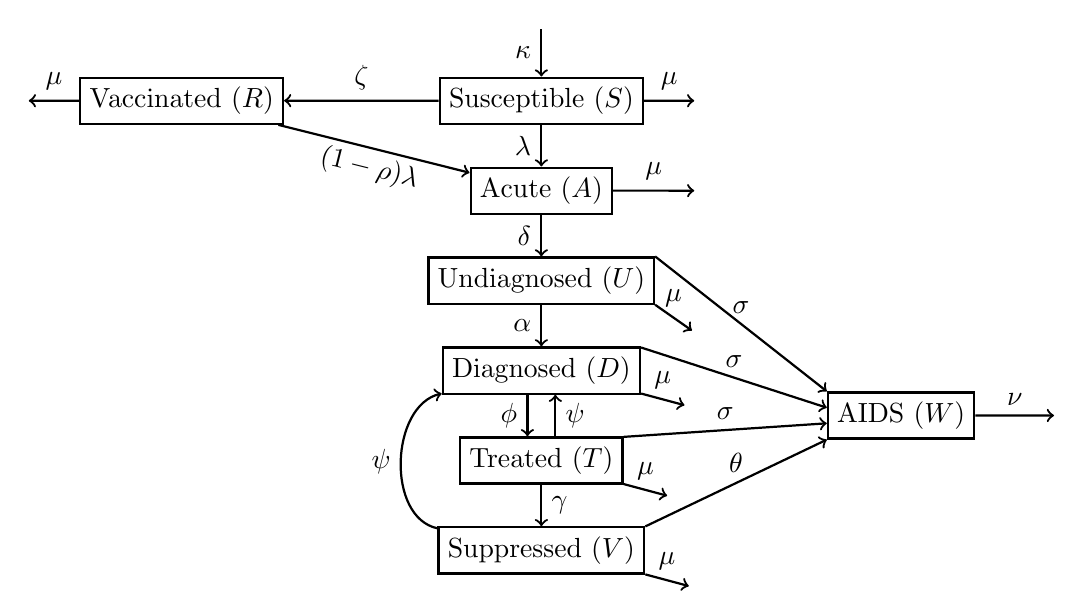
\begin{tikzpicture}[
  thick,
  scale = 1.142,
  compartment/.style = {draw},
  ]

  \node at (0, 5)
  [compartment, name = Susceptible] {Susceptible ($S$)};

  \node at (-4, 5)
  [compartment, name = Vaccinated] {Vaccinated ($R$)};

  \node at (0, 4)
  [compartment, name = Acute] {Acute ($A$)};

  \node at (0, 3)
  [compartment, name = Undiagnosed] {Undiagnosed ($U$)};

  \node at (0, 2)
  [compartment, name = Diagnosed] {Diagnosed ($D$)};

  \node at (0, 1)
  [compartment, name = Treated] {Treated ($T$)};

  \node at (0, 0)
  [compartment, name = Suppressed] {Suppressed ($V$)};

  \node at (4, 1.5)
  [compartment, name = AIDS] {AIDS ($W$)};

  \draw [->] (Susceptible) to node [left] {$\lambda$} (Acute);

  \draw [->] (Susceptible) to node [above] {$\zeta$} (Vaccinated);

  \draw [->] (Vaccinated) to node [sloped, below, yshift = 0.05cm] {$(1 - \rho) \lambda$} (Acute);

  \draw [->] (Acute) to node [left] {$\delta$} (Undiagnosed);

  \draw [->] (Undiagnosed) to node [left] {$\alpha$} (Diagnosed);

  \draw [->] (Diagnosed.240) to node [left] {$\phi$} (Treated.120);

  \draw [->] (Treated.60) to node [right] {$\psi$} (Diagnosed.300);

  \draw [->] (Treated) to node [right] {$\gamma$} (Suppressed);

  \draw [->] (Suppressed) to [out = 168, in = 193] node [left] {$\psi$} (Diagnosed);

  \draw [->] (Undiagnosed.12) to node [above] {$\sigma$} (AIDS.162);

  \draw [->] (Diagnosed.13) to node [above] {$\sigma$} (AIDS.174);

  \draw [->] (Treated.16) to node [above] {$\sigma$} (AIDS.186);

  \draw [->] (Suppressed.13) to node [above] {$\theta$} (AIDS.198);

  \draw [<-] (Susceptible) to node [left] {$\kappa$} +(90: 0.8);

  \draw [->] (Susceptible) to node [above] {$\mu$} +(0: 1.7);

  \draw [->] (Vaccinated) to node [above] {$\mu$} +(0: -1.7);

  \draw [->] (Acute) to node [above] {$\mu$} +(0: 1.7);

  \draw [->] (Undiagnosed.348) to node [above] {$\mu$} +(325: 0.5);

  \draw [->] (Diagnosed.347) to node [above] {$\mu$} +(345: 0.5);

  \draw [->] (Treated.344) to node [above] {$\mu$} +(345: 0.5);

  \draw [->] (Suppressed.347) to node [above] {$\mu$} +(345: 0.5);

  \draw [->] (AIDS) to node [above] {$\nu$} +(0: 1.7);

\end{tikzpicture}


%%% Local Variables:
%%% mode: latex
%%% TeX-master: "supplementary_text"
%%% End:

  \caption{Model diagram.}
\end{figure}


\begin{equation}
  \label{model_eqns}
  \begin{split}
    \frac{\md S}{\md t} &= B N - \lambda S - \zeta S- \mu S,
    \\
     \frac{\md R}{\md t} & = \zeta S - \rho \lambda R - \mu R,
    \\
    \frac{\md A}{\md t} &= \lambda S +\rho \lambda R - \delta A - \mu A,
    \\
    \frac{\md U}{\md t} &= \delta A - \alpha U - \mu U - \sigma U,
    \\
    \frac{\md D}{\md t} &=  \alpha U + \psi T + \psi V
    - \phi D - \mu D - \sigma D,
    \\
    \frac{\md T}{\md t} &= \phi D - \psi T - \gamma T - \mu T
    - \sigma T,
    \\
    \frac{\md V}{\md t} &= \gamma T - \psi V - \mu V - \theta V,
    \\
    \frac{\md W}{\md t} &= \sigma U + \sigma D + \sigma T + \theta V -
    \nu W,
  \end{split}
\end{equation}
with
\begin{equation}
  \label{force_of_infection}
  \begin{split}
    \lambda &= \frac{\beta_A A + \beta_U (U + D + T) + \beta_T V}{N},
    \\
    N &= S + R +  A + U + D + T + V,
    \\
    \beta_x &= c \left[1 - (1 - \tau_x)^n\right]
    \text{ for $x \in \{A, U, T\}$},
    \\
    \tau_T &= (1 - \epsilon) \tau_U.
  \end{split}
\end{equation}

The proportion diagnosed is
\begin{equation}
  p_D = \frac{D + T + V + W}{A + U + D + T + V + W},
\end{equation}
the proportion treated is
\begin{equation}
  p_T = \frac{T + V}{D + T + V + W},
\end{equation}
and the proportion with viral suppression is
\begin{equation}
  p_V = \frac{V}{T + V}.
\end{equation}

The targets for the proportions $p_D$, $p_T$, and $p_V$ are all:
if the initial level $p_x(0)$ is less than $90\%$, it will increase
linearly in the first 5 years and then stay at $90\%$ for the
remaining time; and if the initial level is at $90\%$ or above, it
will stay constant for the whole time:
\begin{equation}
  p_x^*(t)
  = p_x(0) + \left[
    \max\left\{0.9, p_x(0)\right\} - p_x(0)
  \right]
  \min\left\{\frac{t}{5}, 1\right\},
\end{equation}
for $x \in \{D, T, V\}$.


Similarly, the proportion of people vaccinated is
\begin{equation}
P_{V} = \frac{R}{S+R},
\end{equation}

We can implement it in the same way as the other controls. When we begin
vaccination in 2020/2025 the initial vaccination level is 0\%, the it
will increase linearly in the first year and then stay at 50\% for the
remaining time.
\begin{equation}
P^{*}_{V}(t) =
  \begin{cases}
    0 & \text{if $t < 5$ or $10$},
    \\
    0.5  & \text{if $t \geq 5$ or $10$},
  \end{cases}
\end{equation}


\section{Rates that are on when $p_x < p^*_x$}

The rates turn on when the proportions are below the target levels:
\begin{equation}
  \begin{split}
    \alpha(t) &= \alpha_{\max} H\left(p_D^*(t) - p_D(t)\right),
    \\
    \phi(t) &= \phi_{\max} H\left(p_T^*(t) - p_T(t)\right),
    \\
    \psi(t) &= \psi_{\max} H\left(p_V(t) - p_V^*(t)\right),
    \\
    \zeta(t) &= \zeta_{max} H\left(P^{*}_{V}(t)-P_{V}(t)\right),
  \end{split}
\end{equation}
where $H(x)$ is the Heaviside function
\begin{equation}
  H(x) =
  \begin{cases}
    0 & \text{if $x < 0$},
    \\
    1 & \text{if $x > 0$}.
  \end{cases}
\end{equation}

The discontinuity of the Heaviside function makes numerical solution
difficult.  Instead, replace $H$ with the continuous piecewise linear
function
\begin{equation}
  H(x) =
  \begin{cases}
    0 & \text{if $x < 0$},
    \\
    x / \chi & \text{if $0 \leq x \leq \chi$},
    \\
    1 & \text{if $x > \chi$},
  \end{cases}
\end{equation}
with some small value of $\chi$.


\section{Rates that are proportional to the $p_x$'s}

\textit{This hasn't been updated with the AIDS class, $W$.}

Let the rates be proportional to the number of people needed to
achieve the target levels:
\begin{equation}
  \begin{split}
    \alpha^*(t) &= \omega_{\alpha}
    [p_D^*(t) - p_D(t)]
    [A(t) + U(t) + D(t) + T(t) + V(t)],
    \\
    \phi^*(t) &= \omega_{\phi}
    [p_T^*(t) - p_T(t)]
    [D(t) + T(t) + V(t)],
    \\
    \psi^*(t) &= - \omega_{\psi}
    [p_V^*(t) - p_V(t)]
    [D(t) + T(t) + V(t)],
  \end{split}
\end{equation}
and then
\begin{equation}
  \begin{split}
    \alpha(t) &=
    \begin{cases}
      \alpha^*(t) & \text{if $0 \leq \alpha^*(t) \leq 1$},
      \\
      0 & \text{if $\alpha^*(t) < 0$},
      \\
      1 & \text{if $\alpha^*(t) > 1$},
    \end{cases}
    \\
    \phi(t) &=
    \begin{cases}
      \phi^*(t) & \text{if $\phi^*(t) > 0$},
      \\
      0 & \text{if $\phi^*(t) < 0$},
    \end{cases}
    \\
    \psi(t) &=
    \begin{cases}
      \psi^*(t) & \text{if $\psi^*(t) \geq 0$},
      \\
      0 & \text{if $\psi^*(t) < 0$}.
    \end{cases}
  \end{split}
\end{equation}


\section{Forcing exact $p_x$'s}

\textit{This hasn't been updated with the AIDS class, $W$.}

Let
\begin{equation}
  Z =  U + D + T + V,
\end{equation}
so then
\begin{equation}
  \begin{split}
    U &= (1 - p_D) (Z + A) - A,
    \\
    D &= p_D (1 - p_T) (Z + A),
    \\
    T &= p_D p_T (1 - p_V) (Z + A),
    \\
    V &= p_D p_T p_V (Z + A).
  \end{split}
\end{equation}
Thus,
\begin{equation}
  \begin{split}
    \frac{\md S}{\md t} &= B N - \lambda S - \mu S,
    \\
    \frac{\md A}{\md t} &= \lambda S - \delta A - \mu A,
    \\
    \frac{\md Z}{\md t} &= \delta A - \mu Z - \sigma Z
    + (\sigma - \theta) p_D p_T p_V (Z + A),
    \\
    \lambda &= \frac{\beta_A A + \beta_U Z
      - (\beta_U - \beta_T) p_D p_T p_V (Z + A)}{N}.
  \end{split}
\end{equation}


% \section{Forcing exact $p_x$'s}
%%% Not updated for dropped AIDS class %%%
%
% Differentiating the proportion diagnosed with respect to time gives
% \begin{equation}
%   \begin{split}
%     \frac{\md p_D}{\md t}
%     &= \frac{\left(\frac{\md D}{\md t} + \frac{\md T}{\md t} +
%         \frac{\md V}{\md t}\right)
%       \left(D + T + V + U + A\right)
%       - \left(D + T + V\right)
%       \left(\frac{\md D}{\md t} + \frac{\md T}{\md t} + \frac{\md
%         V}{\md t} + \frac{\md U}{\md t} + \frac{\md A}{\md t}\right)}
%     {\left(D + T + V + U + A\right)^2}
%     \\
%     &= \frac{\left(\frac{\md D}{\md t} + \frac{\md T}{\md t} +
%         \frac{\md V}{\md t}\right)
%       \left(U + A\right)
%       - \left(D + T + V\right)
%       \left(\frac{\md U}{\md t} + \frac{\md A}{\md t}\right)}
%     {\left(D + T + V + U + A\right)^2},
%   \end{split}
% \end{equation}
% so
% \begin{equation}
%   \begin{split}
%     \left(D + T + V + U + A\right)^2 \frac{\md p_D}{\md t}
%     &= \left(\frac{\md D}{\md t} + \frac{\md T}{\md t} +
%       \frac{\md V}{\md t}\right)
%     \left(U + A\right)
%     - \left(D + T + V\right)
%     \left(\frac{\md U}{\md t} + \frac{\md A}{\md t}\right)
%     \\
%     &= \left[\alpha \delta A + \rho U
%       - \mu \left(D + T + V\right)\right]
%     \left(U + A\right)
%     \\ & \quad {}
%     - \left(D + T + V + A_D\right)
%     \left[
%       \lambda S - \alpha \delta A - \rho U
%       - \mu (U + A)
%     \right]
%     \\
%     &= \left(\alpha \delta A + \rho U - \sigma A_D\right)
%     \left(U + A\right)
%     \\ & \quad {}
%     - \left(D + T + V + A_D\right)
%     \left(\lambda S - \alpha \delta A - \rho U\right)
%     \\
%     &= \left(\alpha \delta A + \rho U\right)
%     \left(D + T + V + A_D + U + A\right)
%     \\ & \quad {}
%     - \lambda S \left(D + T + V + A_D\right)
%     - \sigma A_D \left(U + A\right),
%   \end{split}
% \end{equation}
% or
% \begin{equation}
%   \label{alpha}
%   \alpha
%   =
%   \frac{\lambda S \left(D + T + V + A_D\right)
%     + \sigma A_D \left(U + A\right)
%     - \rho U \left(D + T + V + A_D + U + A\right)
%     + \left(D + T + V + A_D + U + A\right)^2 \frac{\md p_D}{\md t}}
%   {\delta A \left(D + T + V + A_D + U + A\right)}.
% \end{equation}


% Differentiating the proportion with viral suppression with respect to
% time gives
% \begin{equation}
%   \begin{split}
%     \frac{\md p_V}{\md t}
%     &= \frac{\frac{\md V}{\md t} (T + V) -
%       V \left(\frac{\md T}{\md t} + \frac{\md V}{\md t}\right)}
%     {\left(T + V\right)^2}
%     \\
%     &= \frac{T \frac{\md V}{\md t}
%       - V \frac{\md T}{\md t}}
%     {\left(T + V\right)^2}
%     \\
%     &= \frac{T \left(\gamma T - \theta V - \psi V - \mu V\right)
%       - V \left(\phi D - \rho T - \psi T - \gamma T -  \mu T\right)}
%     {\left(T + V\right)^2}
%     \\
%     &= \frac{\gamma T (T + V) + (\rho - \theta) T V
%       - \phi D V}
%     {\left(T + V\right)^2},
%   \end{split}
% \end{equation}
% so
% \begin{equation}
%   \label{phi}
%   \phi
%   = \frac{\gamma T (T + V) + (\rho - \theta) T V
%     - \left(T + V\right)^2 \frac{\md p_V}{\md t}}
%   {D V}.
% \end{equation}


% Differentiating the proportion treated with respect to time gives
% \begin{equation}
%   \begin{split}
%     \frac{\md p_{T}}{\md t}
%     &= \frac{\left(\frac{\md T}{\md t} + \frac{\md V}{\md t}\right)
%       \left(D + T + V + A_D\right)
%       - \left(T + V\right)
%       \left(\frac{\md D}{\md t} + \frac{\md T}{\md t} + \frac{\md V}{\md t}
%         + \frac{\md A_D}{\md t}\right)}
%     {\left(D + T + V + A_D\right)^2}
%     \\
%     &= \frac{
%       (D + A_D)
%       \left(\frac{\md T}{\md t} + \frac{\md V}{\md t}\right)
%       - \left(T + V\right)
%       \left(\frac{\md D}{\md t} + \frac{\md A_D}{\md t}\right)}
%     {\left(D + T + V + A_D\right)^2},
%   \end{split}
% \end{equation}
% so
% \begin{equation}
%   \begin{split}
%     \left(D + T + V + A_D\right)^2 \frac{\md p_T}{\md t}
%     &= (D + A_D)
%     \left[
%       \phi D - \rho T - \theta V
%       - (\psi + \mu) \left(T + V\right)
%     \right]
%     \\ & \quad {}
%     - \left(T + V\right)
%     \left[
%       \alpha \delta A - \phi D
%       + \rho (U + T)  + \psi \left(T + V\right) + \theta V - \sigma A_D
%       - \mu \left(D + A_D\right)
%     \right]
%     \\
%     &= (D + A_D)
%     \left[
%       \phi D - \rho T - \theta V
%       - \psi \left(T + V\right)
%     \right]
%     \\ & \quad {}
%     - \left(T + V\right)
%     \left[
%       \alpha \delta A - \phi D
%       + \rho (U + T)  + \psi \left(T + V\right) + \theta V - \sigma A_D
%     \right]
%     \\
%     &=
%     \left[\phi D - \theta V - \rho T - \psi \left(T + V\right)\right]
%     (D + T + V + A_D)
%     - \left(\alpha \delta A + \rho U - \sigma A_D \right)
%     \left(T + V\right),
%     \\
%     &=
%     - \alpha \delta A \left(T + V\right)
%     - \psi \left(T + V\right) (D + T + V + A_D)
%     \\ & \quad {}
%     + \left(\phi D - \theta V - \rho T\right)
%     (D + T + V + A_D)
%     - \left(\rho U - \sigma A_D \right)
%     \left(T + V\right),
%   \end{split}
% \end{equation}
% or
% \begin{equation}
%   \label{psi}
%   \psi
%   =
%   \frac{\left(\phi D - \theta V - \rho T\right)
%     (D + T + V + A_D)
%     - \left(\alpha \delta A + \rho U - \sigma A_D \right)
%     \left(T + V\right)
%     - \left(D + T + V + A_D\right)^2 \frac{\md p_T}{\md t}}
%  {\left(T + V\right) \left(D + T + V + A_D\right)},
% \end{equation}
% with $\alpha$ from \eqref{alpha} and $\phi$ from \eqref{phi}.


% The parameters require $\alpha \in [0, 1]$, $\phi \in [0, \infty]$, and $\psi
% \in [0, \infty]$, but these are not guaranteed by the formulas
% (\ref{alpha}, \ref{phi}, \& \ref{psi}) for $\alpha$, $\phi$, and
% $\psi$.


% \section{Optimal control}
%%% Not updated for dropped AIDS class %%%
%
% Find $\alpha(t) \in [0, 1]$, $\phi(t) \in [0, \infty]$, $\psi(t) \in
% [0, \infty]$ that minimize
% \begin{equation}
%   J(\alpha, \phi, \psi) =
%   \frac{1}{2}
%   \int_0^T (p_D^*(t) - p_D(t))^2
%   + (p_T^*(t) - p_T(t))^2
%   + (p_V^*(t) - p_V(t))^2
%   + \xi (\alpha^2 + \phi^2 + \psi^2) \md t.
% \end{equation}

% Let $\vec{x} = \left(S, A, U, D, T, V, A_D\right)^{\mT}$ be the
% state variables,
% $\vec{q} = \left(q_S, q_A, q_U, q_D, q_T, q_V,
%   q_{A_D}\right)^{\mT}$
% be the adjoint variables, and
% $\vec{u} = \left(\alpha, \phi, \psi\right)^{\mT}$ be the controls.

% The Lagrangian is
% \begin{equation}
%   \mathcal{L} =
%   \int_0^T \frac{1}{2} (p_D^*(t) - p_D(t))^2
%   + \frac{1}{2} (p_T^*(t) - p_T(t))^2
%   + \frac{1}{2} (p_V^*(t) - p_V(t))^2
%   + \xi (\alpha^2 + \phi^2 + \psi^2)
%   + \vec{q}^{\mT} \left[\frac{\md \vec{x}}{\md t} -
%     \vec{f}(\vec{x}, t)\right]
%   \md t.
% \end{equation}

% Taking the derivative with respect to $\vec{x}$ gives
% \begin{equation}
%   \frac{\partial \mathcal{L}}{\partial \vec{x}} =
%   \int_0^T
%   - \left(p_D^*(t) - p_D(t)\right) \frac{\partial p_D}{\partial \vec{x}}
%   - \left(p_T^*(t) - p_T(t)\right) \frac{\partial p_T}{\partial \vec{x}}
%   - \left(p_V^*(t) - p_V(t)\right)
%   \frac{\partial p_V}{\partial \vec{x}}
%   -  \frac{\md \vec{q}}{\md t}
%   - \vec{q}^{\mT} \frac{\partial \vec{f}}{\partial \vec{x}}
%   \md t = 0,
% \end{equation}
% so the adjoint equations are
% \begin{equation}
%   \frac{\md \vec{q}}{\md t}
%   =
%   - \left(p_D^* - p_D\right) \frac{\partial p_D}{\partial \vec{x}}
%   - \left(p_T^* - p_T^*\right) \frac{\partial p_T}{\partial \vec{x}}
%   - \left(p_V^* - p_V\right)
%   \frac{\partial p_V}{\partial \vec{x}}
%   - \vec{q}^{\mT} \frac{\partial \vec{f}}{\partial \vec{x}},
% \end{equation}
% or
% \begin{equation}
%   \begin{split}
%     \frac{\md q_S}{\md t}
%     &=
%     \left(q_S - q_A\right) \lambda \left(1 - \frac{S}{N}\right)
%     + q_S \mu,
%     \\
%     \frac{\md q_A}{\md t}
%     &=
%     \left(p_D^* - p_D\right) \frac{p_D}{D + T + V + A_D + U + A}
%     \\ & \quad\quad {}
%     + \left(q_S - q_A\right) \left(\beta_A - \lambda\right) \frac{S}{N}
%     + q_A \mu
%     + (q_A - q_U) (1 - \alpha) \delta
%     + (q_A - q_D) \alpha \delta,
%     \\
%     \frac{\md q_U}{\md t}
%     &=
%     \left(p_D^* - p_D\right) \frac{p_D}{D + T + V + A_D + U + A}
%     \\ & \quad\quad {}
%     + \left(q_S - q_A\right) \left(\beta_U - \lambda\right) \frac{S}{N}
%     + q_U \mu
%     + (q_U - q_{A_D}) \rho,
%     \\
%     \frac{\md q_D}{\md t}
%     &=
%     - \left(p_D^* - p_D\right) \frac{1 - p_D}{D + T + V + A_D + U + A}
%     + \left(p_T^* - p_T\right) \frac{p_T}{D + T + V + A_D}
%     \\ & \quad\quad {}
%     + \left(q_S - q_A\right) \left(\beta_U - \lambda\right) \frac{S}{N}
%     + q_D \mu
%     + (q_D - q_T) \phi
%     + (q_D - q_{A_D}) \rho,
%     \\
%     \frac{\md q_T}{\md t}
%     &=
%     - \left(p_D^* - p_D\right) \frac{1 - p_D}{D + T + V + A_D + U + A}
%     - \left(p_T^* - p_T\right) \frac{1 - p_T}{D + T + V + A_D}
%     \\ & \quad\quad {}
%     + \left(p_V^* - p_V\right) \frac{p_V}{T + V}
%     \\ & \quad\quad {}
%     + \left(q_S - q_A\right) \left(\beta_U - \lambda\right) \frac{S}{N}
%     + q_T \mu
%     + (q_T - q_D) \psi
%     + (q_T - q_V) \gamma
%     + (q_T - q_{A_D}) \rho,
%     \\
%     \frac{\md q_V}{\md t}
%     &=
%     - \left(p_D^* - p_D\right) \frac{1 - p_D}{D + T + V + A_D + U + A}
%     - \left(p_T^* - p_T\right) \frac{1 - p_T}{D + T + V + A_D}
%     \\ & \quad\quad {}
%     - \left(p_V^* - p_V\right) \frac{1 - p_V}{T + V}
%     \\ & \quad\quad {}
%     + \left(q_S - q_A\right) \left(\beta_T - \lambda\right) \frac{S}{N}
%     + q_V \mu
%     + (q_V - q_D) \psi
%     + (q_V - q_{A_D}) \theta,
%     \\
%     \frac{\md q_{A_D}}{\md t}
%     &=
%     - \left(p_D^* - p_D\right) \frac{1 - p_D}{D + T + V + A_D + U + A}
%     + \left(p_T^* - p_T\right) \frac{p_T}{D + T + V + A_D}
%     \\ & \quad\quad {}
%     + \left(q_S - q_A\right) \left(\beta_{A_D} - \lambda\right) \frac{S}{N}
%     + q_{A_D} (\mu + \sigma),
%   \end{split}
% \end{equation}
% with $\vec{q}(T) = \vec{0}$.

% Taking the derivative with respect to $\vec{u}$ gives
% \begin{equation}
%   \frac{\partial \mathcal{L}}{\partial \vec{u}} =
%   \int_0^T
%   - \vec{q}^{\mT} \frac{\partial \vec{f}}{\partial \vec{u}}
%   + \xi \vec{u}
%   \; \md t = 0,
% \end{equation}
% so the optimality conditions are
% \begin{equation}
%   \vec{u} = \frac{1}{\xi} \vec{q}^{\mT}
%   \frac{\partial \vec{f}}{\partial \vec{u}},
% \end{equation}
% which is
% \begin{equation}
%   \begin{aligned}
%     \alpha &= \frac{1}{\xi} \delta A (q_U - q_D),
%     \\
%     \phi &= \frac{1}{\xi} D (q_D - q_T),
%     \\
%     \psi &= \frac{1}{\xi} [T (q_T - q_D) + V (q_V - q_D)].
%   \end{aligned}
% \end{equation}
% Then the optimality condition is
% \begin{equation}
%   \begin{aligned}
%     \alpha^* &=
%     \begin{cases}
%       0 & \text{if $\alpha < 0$},
%       \\
%       1 & \text{if $\alpha > 1$},
%       \\
%       \alpha & \text{otherwise},
%     \end{cases}
%     \\
%     \phi^* &=
%     \begin{cases}
%       0 & \text{if $\phi < 0$},
%       \\
%       \phi & \text{otherwise},
%     \end{cases}
%     \\
%     \psi^* &=
%     \begin{cases}
%       0 & \text{if $\psi < 0$},
%       \\
%       \psi & \text{otherwise}.
%     \end{cases}
%   \end{aligned}
% \end{equation}


% \section{Scratch}

% A kind of moving average is
% \begin{equation}
%   z = \frac{\int_0^t \me^{-\xi (t - s)} p(s) \md s}
%   {\int_0^t \me^{-\xi (t - s)} \md s}
%   = \frac{\int_0^t \me^{\xi s} p(s) \md s}
%   {\int_0^t \me^{\xi s} \md s}
%   = \xi \frac{\int_0^t \me^{\xi s} p(s) \md s}
%   {\me^{\xi t} - 1},
% \end{equation}
% so
% \begin{equation}
%   \begin{split}
%     \frac{\md z}{\md t} &=
%     \xi
%     \frac{\me^{\xi t} p(t) (\me^{\xi t} - 1)
%       - \xi \me^{\xi t} \int_0^t \me^{\xi s} p(s) \md s}
%     {(\me^{\xi t} - 1)^2}
%     \\
%     &=
%     \xi \me^{\xi t}
%     \left[
%       \frac{p(t)}{\me^{\xi t} - 1}
%       - \xi \frac{\int_0^t \me^{\xi s} p(s) \md s}
%       {(\me^{\xi t} - 1)^2}
%     \right]
%     \\
%     &=
%     \xi \me^{\xi t}
%     \left[
%       \frac{p(t)}{\me^{\xi t} - 1}
%       - \frac{z}{\me^{\xi t} - 1}
%     \right]
%     \\
%     &=
%     \xi \frac{p(t) - z}{1 - \me^{-\xi t}}
%   \end{split}
% \end{equation}


\end{document}
